% Week 5: Transformers - The Speed Revolution
% NLP Course 2025
% Created: 2025-10-03
% Pedagogical enhancements: Discovery opening, BSc boxes, checkpoint quizzes
% Framework: Hope → Disappointment → Breakthrough
% Template: Lavender/Purple styling from template_beamer_final.tex

\documentclass[8pt,aspectratio=169]{beamer}
\usetheme{Madrid}
\usecolortheme{seahorse}
\setbeamertemplate{navigation symbols}{}

% Color definitions (lavender/purple palette)
\definecolor{mlblue}{RGB}{0,102,204}
\definecolor{mlpurple}{RGB}{51,51,178}
\definecolor{mllavender}{RGB}{173,173,224}
\definecolor{mllavender2}{RGB}{193,193,232}
\definecolor{mllavender3}{RGB}{204,204,235}
\definecolor{mllavender4}{RGB}{214,214,239}
\definecolor{mlorange}{RGB}{255,127,14}
\definecolor{mlgreen}{RGB}{44,160,44}
\definecolor{mlred}{RGB}{214,39,40}

% Apply colors to Madrid theme
\setbeamercolor{palette primary}{bg=mllavender3,fg=mlpurple}
\setbeamercolor{palette secondary}{bg=mllavender2,fg=mlpurple}
\setbeamercolor{palette tertiary}{bg=mllavender,fg=white}
\setbeamercolor{palette quaternary}{bg=mlpurple,fg=white}
\setbeamercolor{structure}{fg=mlpurple}
\setbeamercolor{section in toc}{fg=mlpurple}
\setbeamercolor{subsection in head/foot}{bg=mllavender3,fg=mlpurple}
\setbeamercolor{frametitle}{fg=mlpurple,bg=mllavender3}
\setbeamercolor{title}{fg=mlpurple}
\setbeamercolor{item}{fg=mlpurple}

% Custom commands
\newcommand{\bottomnote}[1]{%
\vfill
\vspace{-2mm}
\textcolor{mllavender2}{\rule{\textwidth}{0.4pt}}
\vspace{1mm}
\footnotesize
\textbf{#1}
}

\newcommand{\highlight}[1]{\textcolor{mlpurple}{\textbf{#1}}}
\newcommand{\success}[1]{\textcolor{mlgreen}{\textbf{#1}}}
\newcommand{\warning}[1]{\textcolor{mlred}{\textbf{#1}}}
\newcommand{\keypoint}[1]{\textcolor{mlpurple}{\textbf{#1}}}

% BSc Pedagogical boxes (matching Week 3 & Week 4)
\usepackage{tcolorbox}

\newtcolorbox{checkpoint}[1][]{
    colback=yellow!10!white,
    colframe=yellow!75!black,
    title=\textbf{Checkpoint: #1},
    fonttitle=\bfseries,
    left=3pt, right=3pt, top=3pt, bottom=3pt
}

\newtcolorbox{intuition}[1][]{
    colback=purple!5!white,
    colframe=purple!75!black,
    title=\textbf{Intuition: #1},
    fonttitle=\bfseries,
    left=3pt, right=3pt, top=3pt, bottom=3pt
}

\newtcolorbox{realworld}[1][]{
    colback=orange!5!white,
    colframe=orange!75!black,
    title=\textbf{Real World: #1},
    fonttitle=\bfseries,
    left=3pt, right=3pt, top=3pt, bottom=3pt
}

% Math and code support
\usepackage{amsmath,amssymb}
\usepackage{listings}
\usepackage{tikz}

\lstset{
    basicstyle=\ttfamily\small,
    breaklines=true,
    frame=single,
    backgroundcolor=\color{mllavender4}
}

\title{Natural Language Processing}
\subtitle{Week 5: The Speed Revolution}
\author{From Sequential Waiting to Parallel Processing}
\date{NLP Course 2025}

\begin{document}

% Title slide
\begin{frame}
\titlepage
\end{frame}

% ============================================
% NEW SLIDE 2: DISCOVERY-BASED OPENING
% ============================================

\begin{frame}{Before We Begin: A Thought Experiment}
    \begin{center}
    \textbf{\Large Imagine You're Designing a GPU-Friendly Neural Network}
    \end{center}

    \vspace{1em}
    \begin{columns}[T]
        \begin{column}{0.55\textwidth}
            \textbf{Your Challenge:}

            You have an expensive NVIDIA A100 GPU:
            \begin{itemize}
                \item 5,120 processors (CUDA cores)
                \item All capable of working simultaneously
                \item Cost: \$10,000
            \end{itemize}

            \vspace{0.5em}
            \textbf{The Problem:}
            \begin{itemize}
                \item Current RNN processes words sequentially
                \item Only 49 cores active, 5,071 cores idle (1\% utilization!)
                \item Training takes 90 days
            \end{itemize}

            \vspace{1em}
            \textbf{Design Constraints:}
            \begin{enumerate}
                \item Must process sequences (word order matters!)
                \item Must use ALL 5,120 processors simultaneously
                \item Cannot wait for previous word to finish
                \item Must preserve position information
            \end{enumerate}

            \vspace{1em}
            \colorbox{orange!10}{\parbox{0.95\columnwidth}{
                \textbf{Imagine:} Your RNN takes 90 days to train\\
                \textbf{Question:} If you could use ALL 5,120 cores simultaneously, how long?\\
                \textbf{Think about:}
                \begin{itemize}
                    \item Currently: 49 cores = 90 days
                    \item Could use: 5,120 cores (100x more)
                    \item 100x speedup = ? days
                \end{itemize}
            }}
        \end{column}

        \begin{column}{0.43\textwidth}
            \textbf{Your Design:}

            \vspace{0.5em}
            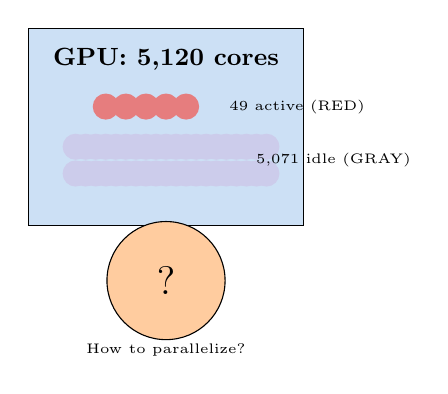
\begin{tikzpicture}[scale=0.85, every node/.style={font=\small}]
                % GPU visualization
                \node[draw, rectangle, minimum width=3.5cm, minimum height=2.5cm, fill=mlblue!20] at (0, 1.5) {};
                \node at (0, 2.5) {\textbf{GPU: 5,120 cores}};

                % Sequential bottleneck
                \foreach \i in {1,...,5} {
                    \node[circle, fill=mlred!60, minimum size=0.15cm] at (-1.2+0.3*\i, 1.8) {};
                }
                \node[right, font=\tiny] at (0.8, 1.8) {49 active (RED)};

                % Idle cores
                \foreach \i in {1,...,20} {
                    \node[circle, fill=mllavender3, minimum size=0.15cm] at (-1.5+0.15*\i, 1.2) {};
                }
                \foreach \i in {1,...,20} {
                    \node[circle, fill=mllavender3, minimum size=0.15cm] at (-1.5+0.15*\i, 0.8) {};
                }
                \node[right, font=\tiny] at (1.2, 1.0) {5,071 idle (GRAY)};

                % Question mark for solution
                \node[draw, circle, fill=mlorange!40, minimum size=1.5cm] at (0, -0.8) {\Large ?};
                \node[below, font=\tiny] at (0, -1.6) {How to parallelize?};
            \end{tikzpicture}

            \vspace{1em}
            \textbf{Key Questions:}
            \begin{itemize}
                \item How do you process all words at once?
                \item How do you preserve word order?
                \item What's the architectural change needed?
            \end{itemize}
        \end{column}
    \end{columns}

    \bottomnote{Next slide reveals: Your design IS the transformer architecture!}
\end{frame}

% ============================================
% NEW SLIDE 3: TABLE OF CONTENTS
% ============================================

\begin{frame}{Table of Contents}
    \tableofcontents
\end{frame}

% ============================================
% PART 1: THE WAITING GAME (5 slides)
% ============================================

\section{The Waiting Game}

\begin{frame}[t]
\vfill
\centering
\begin{beamercolorbox}[sep=8pt,center]{title}
\usebeamerfont{title}\Large The Waiting Game
\end{beamercolorbox}
\vfill
\end{frame}

% Slide 1: The Nightmare Scenario (ENHANCED)
\begin{frame}[t]{The Nightmare Scenario}
\textbf{From human experience: Imagine waiting 4 years for your model to train}

\vspace{5mm}
\begin{itemize}
    \item Your research would stop
    \item Competitors would publish first
    \item No iterations, no experiments
    \item This was the reality in 2016
\end{itemize}

\vspace{8mm}
\textbf{The Data:}
\begin{itemize}
\item English Wikipedia: 6 billion words
\item Need to process every word, many times
\item Training typically requires 10-20 epochs
\item Total words to process: 60-120 billion
\end{itemize}

\vspace{8mm}
\textbf{With an RNN on modern GPU - Let's calculate:}
\begin{itemize}
\item Processing speed: ~800 words/second
\item Calculate: $\frac{100\text{ billion words}}{800 \text{ words/sec}} = 125\text{ million seconds}$
\item Converting to days: $125{,}000{,}000 \div 86{,}400 = 1{,}447$ days
\item \highlight{3.9 years of continuous training}
\end{itemize}

\vspace{8mm}
\begin{center}
\warning{\textbf{The Waiting Game:} Press ``train'', come back in 2027}
\end{center}

\vspace{5mm}
\begin{center}
\includegraphics[width=0.85\textwidth]{../figures/sr_01_training_time_comparison.pdf}
\end{center}

\bottomnote{Even with parallelization tricks, you're looking at months of waiting}
\end{frame}

% Slide 2: Why So Slow? (ENHANCED with analogy FIRST)
\begin{frame}[t]{Why So Slow? The Sequential Trap}
\textbf{Human analogy FIRST:}

\vspace{5mm}
Imagine a factory with 5,000 workers:
\begin{itemize}
    \item Task 1: Worker A assembles part, Worker B waits
    \item Task 2: Worker B adds component, Worker C waits
    \item Task 3: Worker C finishes product, Workers D-Z wait
    \item 4,997 workers standing idle, getting paid to do nothing
\end{itemize}

\vspace{8mm}
\textbf{This is exactly what RNN does:}

\vspace{5mm}
Step 1: Process ``The'' → hidden state $h_1$\\
Step 2: Wait for $h_1$, process ``cat'' → hidden state $h_2$\\
Step 3: Wait for $h_2$, process ``sat'' → hidden state $h_3$\\
\hspace{2cm} $\vdots$

\vspace{8mm}
\textbf{Your GPU Has:}
\begin{itemize}
\item 5,120 CUDA cores (NVIDIA A100)
\item Can perform 5,120 operations \textit{simultaneously}
\item But RNN uses only ONE core at a time
\item The other 5,119 sit idle, waiting
\end{itemize}

\vspace{8mm}
\begin{intuition}[Assembly Line Waste]
Sequential processing = paying 5,000 workers but only letting one work at a time. The bottleneck isn't compute power - it's the sequential dependency!
\end{intuition}

\vspace{5mm}
\begin{center}
\includegraphics[width=0.9\textwidth]{../figures/sr_03_sequential_bottleneck.pdf}
\end{center}

\bottomnote{Sequential processing forces massive underutilization of parallel hardware}
\end{frame}

% Slide 3: GPU Bored to Death (ENHANCED with actual specs)
\begin{frame}[t]{Your \$10,000 GPU Is 99\% Idle}
\begin{center}
\textbf{Actual GPU Utilization During RNN Training}
\end{center}

\vspace{5mm}
\begin{columns}[T]
\column{0.48\textwidth}
\textbf{The Hardware (NVIDIA A100):}
\begin{center}
\begin{tabular}{|l|c|}
\hline
\textbf{Specification} & \textbf{Value} \\
\hline
Price & \$10,000 \\
CUDA Cores & 5,120 \\
Tensor Cores & 432 \\
Peak Performance & 312 TFLOPS \\
Memory Bandwidth & 1.6 TB/s \\
Design Purpose & Massive parallelism \\
\hline
\end{tabular}
\end{center}

\vspace{5mm}
\textbf{What RNN Actually Uses:}
\begin{itemize}
\item Active processors: 49
\item Idle processors: 5,071
\item Utilization: \highlight{0.96\%}
\item Actual throughput: 3 TFLOPS
\item Efficiency: 1\% of potential
\end{itemize}

\column{0.48\textwidth}
\textbf{The Cost:}
\begin{itemize}
\item You paid: \$10,000
\item You're getting: \$96 worth of compute
\item Wasted capacity: 99.04\%
\item Like buying a sports car for city traffic
\end{itemize}

\vspace{5mm}
\textbf{Visualization:}\\
Imagine 5,120 workers at a factory:
\begin{itemize}
    \item 49 working (0.96\%)
    \item 5,071 standing around waiting (99.04\%)
    \item All getting paid the same
    \item All day, every day, for 90 days
\end{itemize}

\vspace{5mm}
\textbf{Financial Impact:}
\begin{itemize}
    \item 90-day training: \$45,000 cloud cost
    \item 99\% wasted: \$44,550 thrown away
    \item Could be: 100x faster, \$450 cost
\end{itemize}
\end{columns}

\vspace{10mm}
\begin{center}
\warning{\textbf{The Waste:} This is like hiring 100 people but only giving work to 1}
\end{center}

\vspace{5mm}
\begin{center}
\includegraphics[width=0.85\textwidth]{../figures/sr_02_gpu_utilization_waste.pdf}
\end{center}

\bottomnote{Modern GPUs are designed for parallelism - sequential processing wastes their power}
\end{frame}

% Slide 4: Attention Helped... A Little
\begin{frame}[t]{Week 4 Recap: Attention Helped... A Little}
\textbf{What We Learned Last Week:}

\vspace{5mm}
\textbf{RNN Alone:}
\begin{itemize}
\item All history compressed into one vector
\item Long sequences: information lost
\item Translation quality: BLEU 18.5
\item Training time: 90 days for large model
\end{itemize}

\vspace{8mm}
\textbf{RNN + Attention:}
\begin{itemize}
\item Keep all encoder states
\item Decoder selectively attends
\item Translation quality: BLEU 33.2 (\textcolor{green}{+79\% improvement})
\item Training time: 45 days (\textcolor{green}{2x faster})
\end{itemize}

\vspace{8mm}
\textbf{But...}
\begin{itemize}
\item Still sequential processing (RNN part)
\item Still waiting for previous words
\item GPU utilization: 5\% (slightly better, but still terrible)
\item 45 days is better than 90, but still \textit{months}
\end{itemize}

\vspace{8mm}
\begin{center}
\keypoint{Quality improved, but speed problem remains}
\end{center}

\bottomnote{Attention solved the bottleneck problem but not the speed problem}
\end{frame}

% Slide 5: Quantifying the Problem (ENHANCED - Chart 1)
\begin{frame}[t]{Quantifying the Speed Problem}
\begin{columns}[T]
\column{0.48\textwidth}
\textbf{Training Time Comparison}

\vspace{3mm}
\begin{tabular}{|l|c|c|}
\hline
\textbf{Model} & \textbf{Days} & \textbf{GPU} \\
\hline
RNN & 90 & 1\% \\
RNN+Att. & 45 & 5\% \\
\textcolor{green}{\textbf{Target}} & \textcolor{green}{\textbf{1}} & \textcolor{green}{\textbf{90\%}} \\
\hline
\end{tabular}

\vspace{5mm}
\textbf{The Bottleneck:}
\begin{itemize}
\item RNN: Sequential = $O(n)$
\item Target: Parallel = $O(1)$
\item Potential: \textbf{100x speedup}
\end{itemize}

\vspace{5mm}
\textbf{Key Question:}\\
\highlight{Can we keep attention but eliminate sequential processing?}

\column{0.48\textwidth}
\begin{center}
\includegraphics[width=0.95\columnwidth]{../figures/sr_18_complexity_comparison.pdf}
\end{center}
\end{columns}

\bottomnote{Complexity comparison shows the path: Remove sequential dependency → Unlock parallelization}
\end{frame}

% NEW SLIDE 5.5: Timeline - Historical Context
\begin{frame}[t]{Historical Context: The Speed Crisis (2014-2017)}
\textbf{Timeline of the Speed Problem:}

\vspace{5mm}
\begin{center}
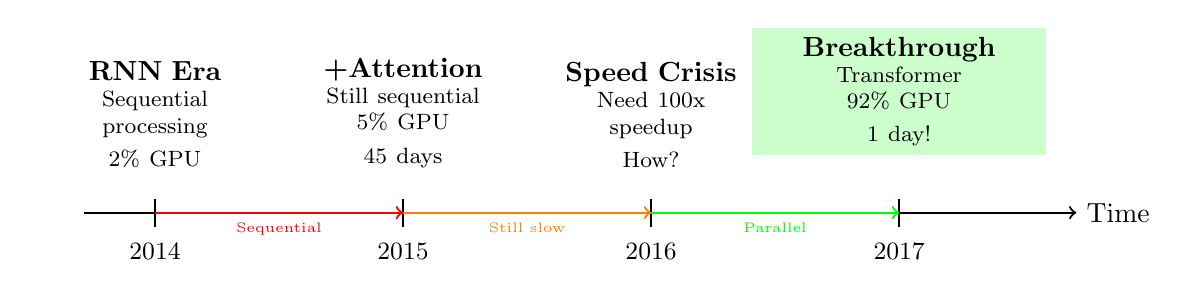
\begin{tikzpicture}[scale=0.9]
% Timeline axis
\draw[thick, ->] (0,0) -- (14,0) node[right] {Time};

% 2014: RNN dominance
\draw[thick] (1,-0.2) -- (1,0.2);
\node[below] at (1,-0.3) {\small 2014};
\node[above, text width=3cm, align=center] at (1,0.5) {\textbf{RNN Era}\\{\footnotesize Sequential\\processing\\2\% GPU}};

% 2015: Attention added
\draw[thick] (4.5,-0.2) -- (4.5,0.2);
\node[below] at (4.5,-0.3) {\small 2015};
\node[above, text width=3cm, align=center] at (4.5,0.5) {\textbf{+Attention}\\{\footnotesize Still sequential\\5\% GPU\\45 days}};

% 2016: Speed crisis
\draw[thick] (8,-0.2) -- (8,0.2);
\node[below] at (8,-0.3) {\small 2016};
\node[above, text width=3cm, align=center] at (8,0.5) {\textbf{Speed Crisis}\\{\footnotesize Need 100x\\speedup\\How?}};

% 2017: Transformer
\draw[thick] (11.5,-0.2) -- (11.5,0.2);
\node[below] at (11.5,-0.3) {\small 2017};
\node[above, text width=3.5cm, align=center, fill=green!20] at (11.5,0.8) {\textbf{Breakthrough}\\{\footnotesize Transformer\\92\% GPU\\1 day!}};

% Annotation arrows
\draw[red, thick, ->] (1,0) -- (4.5,0) node[midway, below] {\tiny Sequential};
\draw[orange, thick, ->] (4.5,0) -- (8,0) node[midway, below] {\tiny Still slow};
\draw[green, thick, ->] (8,0) -- (11.5,0) node[midway, below] {\tiny Parallel};
\end{tikzpicture}
\end{center}

\vspace{5mm}
\textbf{The Challenge (2014-2016):}
\begin{itemize}
\item Models getting larger (10M → 200M parameters)
\item Sequential processing = linear time scaling
\item GPU mostly idle (cannot parallelize)
\item Research question: \textit{How to break the sequential bottleneck?}
\end{itemize}

\bottomnote{Timeline shows: 3 years of speed crisis led to transformer breakthrough in 2017}
\end{frame}

% ============================================
% PART 2: ATTENTION WITHOUT RNN (6 slides)
% ============================================

\section{The First Attempt}

\begin{frame}[t]
\vfill
\centering
\begin{beamercolorbox}[sep=8pt,center]{title}
\usebeamerfont{title}\Large The First Attempt
\end{beamercolorbox}
\vfill
\end{frame}

% Slide 6: The Radical Idea
% Slide 6: The Radical Idea: Pure Attention (VISUAL - CHANGE 3)
\begin{frame}[t]{The Radical Idea: Pure Attention}
\textbf{The Hypothesis:}
\begin{center}
``What if every word directly attends to every other word?''
\end{center}

\vspace{3mm}
\begin{center}
\includegraphics[width=0.95\textwidth]{../figures/sr_15_architecture_comparison.pdf}
\end{center}

\vspace{3mm}
\begin{center}
\keypoint{Remove the sequential bottleneck → 100x speedup}
\end{center}

\bottomnote{Old way: 1-5\% GPU utilization with waiting. New way: 85-92\% GPU utilization with full parallelization}
\end{frame}

% Slide 7: THE FIRST SUCCESS
\begin{frame}[t]{The First Success: Short Sentences Work Great!}
\begin{center}
\textbf{Early Experiments (2017): Testing Pure Attention}
\end{center}

\vspace{5mm}
\textbf{Test Cases (10-20 word sentences):}

\vspace{5mm}
\begin{tabular}{|l|l|c|}
\hline
\textbf{English} & \textbf{French (Pure Attention)} & \textbf{Quality} \\
\hline
The cat sat & Le chat s'est assis & \textcolor{green}{Perfect!} \\
I love you & Je t'aime & \textcolor{green}{Perfect!} \\
Good morning everyone & Bonjour tout le monde & \textcolor{green}{Perfect!} \\
\hline
\end{tabular}

\vspace{10mm}
\textbf{Performance Metrics:}
\begin{columns}[T]
\column{0.48\textwidth}
\textbf{Quality:}
\begin{itemize}
\item BLEU score: 32.1
\item Same as RNN+Attention!
\item No quality loss
\end{itemize}

\column{0.48\textwidth}
\textbf{Speed:}
\begin{itemize}
\item Training time: \textcolor{green}{\textbf{10x faster}}
\item GPU utilization: 45\%
\item Massive improvement!
\end{itemize}
\end{columns}

\vspace{10mm}
\begin{center}
\success{\textbf{Breakthrough Moment:} Attention works without RNN! And it's FAST!}
\end{center}

\vspace{5mm}
\begin{center}
\includegraphics[width=0.65\textwidth]{../figures/sr_04_attention_success_short.pdf}
\end{center}

\bottomnote{The research team was ecstatic - looked like the solution}
\end{frame}

% Slide 8: THE FAILURE PATTERN EMERGES (ENHANCED with BSc box)
\begin{frame}[t]{The Failure Pattern Emerges}
\begin{center}
\textbf{Testing on Longer Sequences... Disaster Strikes}
\end{center}

\vspace{5mm}
\textbf{Experimental Results (Vaswani et al., 2017 - before positional encoding):}

\vspace{5mm}
\begin{tabular}{|l|c|c|c|}
\hline
\textbf{Sequence Length} & \textbf{BLEU Score} & \textbf{Quality Drop} & \textbf{Training Speed} \\
\hline
10 words & 32.1 & Baseline & 10x faster \\
20 words & 31.8 & -1\% & 10x faster \\
50 words & 18.4 & \textcolor{red}{-43\%} & 10x faster \\
100 words & 8.2 & \textcolor{red}{-74\%} & 10x faster \\
200 words & 3.1 & \textcolor{red}{-90\%} & 10x faster \\
\hline
\end{tabular}

\vspace{10mm}
\textbf{The Pattern:}
\begin{itemize}
\item Short sequences: Works perfectly
\item Long sequences: Complete collapse
\item Speed: Consistently fast (good news)
\item Quality: Degrades catastrophically with length (bad news)
\end{itemize}

\vspace{8mm}
\begin{checkpoint}[Understanding the Position Problem]
\textbf{Quick Check:} Why does pure attention fail on long sequences?

\vspace{0.3em}
\textbf{Answer:} Pure attention treats all word orderings as identical - it's permutation invariant. "The cat sat" and "sat cat The" produce the same outputs. Without RNN sequential processing, we lost position information!
\end{checkpoint}

\vspace{5mm}
\begin{center}
\includegraphics[width=0.85\textwidth]{../figures/sr_05_quality_degradation.pdf}
\end{center}

\bottomnote{Real-world sentences are often 20-50+ words - this was unusable}
\end{frame}

% Slide 9: DIAGNOSING THE PROBLEM
\begin{frame}[t]{Diagnosing the Root Cause}
\textbf{Let's trace what happens with: ``The cat sat on the mat''}

\vspace{5mm}
\textbf{With RNN+Attention:}
\begin{itemize}
\item RNN processes: ``The'' (position 1), ``cat'' (position 2), ``sat'' (position 3)...
\item Hidden states carry position information automatically
\item Model knows ``cat'' comes before ``sat''
\item Order preserved naturally
\end{itemize}

\vspace{8mm}
\textbf{With Pure Attention (No RNN):}
\begin{itemize}
\item All words process simultaneously
\item ``cat'' attends to ``sat'', ``the'', ``mat''...
\item But: \textcolor{red}{No way to tell which word came first!}
\item These are identical to pure attention:
\begin{itemize}
\item ``The cat sat on the mat''
\item ``The mat sat on the cat'' \textcolor{red}{← Wrong meaning!}
\item ``Cat the sat mat on the'' \textcolor{red}{← Nonsense!}
\end{itemize}
\end{itemize}

\vspace{8mm}
\begin{center}
\textbf{Root Cause Identified:}
\end{center}

\vspace{3mm}
\warning{\textbf{Attention is permutation invariant} - order doesn't matter!}

\vspace{5mm}
\begin{center}
\includegraphics[width=0.85\textwidth]{../figures/sr_06_permutation_invariance.pdf}
\end{center}

\bottomnote{Without RNN, we lost the sequence information that tells us word order}
\end{frame}

% Slide 10: What Information Got Lost? (VISUAL - CHANGE 1)
\begin{frame}[t]{What Information Got Lost?}
\begin{center}
\includegraphics[width=0.95\textwidth]{../figures/sr_13_attention_capabilities_infographic.pdf}
\end{center}

\vspace{5mm}
\begin{center}
\keypoint{Attention is permutation invariant - order doesn't matter!}
\end{center}

\bottomnote{Visual summary: Pure attention sees meaning but not position}
\end{frame}

% Slide 11: The Position Problem → Solution (VISUAL MERGE - CHANGE 2)
% Merges old Slides 10+11 into single visual
\begin{frame}[t]{The Position Problem: Diagnosis \& Solution}
\begin{center}
\includegraphics[width=0.95\textwidth]{../figures/sr_14_position_problem_solution.pdf}
\end{center}

\vspace{3mm}
\begin{center}
\keypoint{Solution: Position as added signal, not sequential process}
\end{center}

\bottomnote{From problem to solution: Four requirements guide the positional encoding design}
\end{frame}

% ============================================
% NEW SLIDE 11A: CHECKPOINT QUIZ 1
% ============================================

\begin{frame}{Checkpoint: Understanding the Bottleneck}
\begin{center}
\textbf{Test Your Understanding}
\end{center}

\vspace{5mm}
\begin{columns}[T]
\column{0.48\textwidth}
\textbf{Quick Quiz:}

\vspace{3mm}
\textbf{Question 1:} Why can't pure attention (without RNN) tell word order?

\begin{itemize}
\item[A)] Not enough parameters
\item[B)] Permutation invariant - treats all orderings equally
\item[C)] Softmax function issue
\item[D)] Embedding dimensions too small
\end{itemize}

\vspace{8mm}
\textbf{Question 2:} What information does positional encoding add?

\begin{itemize}
\item[A)] Word meanings
\item[B)] Unique position signature for each location
\item[C)] Grammar rules
\item[D)] Translation pairs
\end{itemize}

\column{0.48\textwidth}
\textbf{Answers:}

\vspace{3mm}
\textbf{Answer 1:} B - Permutation invariant

\vspace{0.5em}
Attention weights don't change if you shuffle input order. ``cat sat'' and ``sat cat'' produce identical attention patterns because attention is based on content similarity, not position.

\vspace{8mm}
\textbf{Answer 2:} B - Unique position signature

\vspace{0.5em}
Each position gets a unique sine/cosine pattern added to its embedding. Position 1 has a different pattern than Position 2. This allows the model to distinguish word order without sequential processing.
\end{columns}

\vspace{8mm}
\begin{center}
\keypoint{Position must be explicit when processing is parallel!}
\end{center}
\end{frame}

% ============================================
% PART 3: THE BREAKTHROUGH (10 slides)
% ============================================

\section{The Positional Encoding Revolution}

\begin{frame}[t]
\vfill
\centering
\begin{beamercolorbox}[sep=8pt,center]{title}
\usebeamerfont{title}\Large The Positional Encoding Revolution
\end{beamercolorbox}
\vfill
\end{frame}

% Slide 12: HUMAN INTROSPECTION (ENHANCED - Chart 2)
\begin{frame}[t]{Human Introspection: How Do YOU Know Order?}
\textbf{Prompt: When you read, how do you track word position?}

\vspace{3mm}
\begin{center}
\includegraphics[width=0.90\textwidth]{../figures/sr_19_human_reading_pattern.pdf}
\end{center}

\vspace{3mm}
\begin{intuition}[Timestamps in Reading]
When you read, position works like timestamps on photos. Each word has BOTH content (what it means) AND location (where it is). You don't process them separately - they're fused together in your understanding!
\end{intuition}

\vspace{3mm}
\textbf{Key insight:} What if we add a ``position number'' to each word's meaning vector?

\bottomnote{Visual shows: Spatial layout (eyes) + Mental counting (numbers) = Combined understanding}
\end{frame}

% Slide 13: THE HYPOTHESIS
\begin{frame}[t]{The Hypothesis: Position as Added Signal}
\begin{center}
\textbf{Conceptual Idea (No Math Yet)}
\end{center}

\vspace{8mm}
\textbf{The Approach:}
\begin{itemize}
\item Each word has a meaning vector: [0.3, 0.5, 0.1, ...]
\item Create a position pattern: [0.1, 0.0, 0.05, ...]
\item Add them together: [0.4, 0.5, 0.15, ...]
\item Now word has \textit{both} meaning and position!
\end{itemize}

\vspace{10mm}
\begin{columns}[T]
\column{0.48\textwidth}
\textbf{Why This Should Work:}
\begin{itemize}
\item Position 1 gets pattern A
\item Position 2 gets pattern B
\item Position 3 gets pattern C
\item Each position unique
\item Model sees combined signal
\end{itemize}

\column{0.48\textwidth}
\textbf{Analogy:}\\
Like adding GPS coordinates to photos:
\begin{itemize}
\item Photo content = meaning
\item GPS tag = position
\item Together = complete info
\item Can process in parallel
\end{itemize}
\end{columns}

\vspace{10mm}
\begin{center}
\textbf{Two-Column Comparison:}
\end{center}

\vspace{3mm}
\begin{tabular}{|l|l|}
\hline
\textbf{Old Way (RNN)} & \textbf{New Way (Positional Encoding)} \\
\hline
Process sequentially to get position & Add position signal to embedding \\
Position emerges from order & Position explicitly encoded \\
Must wait for previous words & All positions computed in parallel \\
\hline
\end{tabular}

\bottomnote{Key insight: Position can be a feature, not a process!}
\end{frame}

% Slide 14: ZERO-JARGON EXPLANATION (ENHANCED - Chart 3)
\begin{frame}[t]{Zero-Jargon Explanation: Adding Position Numbers}
\textbf{Example: The word ``cat'' at position 2}

\vspace{3mm}
\begin{center}
\includegraphics[width=0.95\textwidth]{../figures/sr_20_vector_addition_bars.pdf}
\end{center}

\vspace{3mm}
\textbf{The Magic:}
\begin{itemize}
\item Embedding (blue) = meaning of word
\item Position (orange) = location in sentence
\item Combined (stacked) = complete representation
\item All computed in parallel - no waiting!
\end{itemize}

\vspace{3mm}
\begin{center}
\highlight{This is called ``positional encoding''}
\end{center}

\bottomnote{Visual shows: Embedding + Position = Combined vector with both meaning and location}
\end{frame}

% Slide 15: GEOMETRIC INTUITION (ENHANCED with BSc box)
\begin{frame}[t]{Geometric Intuition: Sine Wave Patterns}
\textbf{How to create unique patterns for each position?}

\vspace{8mm}
\textbf{Start in 2D (easy to visualize):}

\vspace{5mm}
\begin{columns}[T]
\column{0.48\textwidth}
\textbf{The Idea:}
\begin{itemize}
\item Position 1: [sin(1), cos(1)] = [0.84, 0.54]
\item Position 2: [sin(2), cos(2)] = [0.91, -0.42]
\item Position 3: [sin(3), cos(3)] = [0.14, -0.99]
\item Each position: unique 2D point
\end{itemize}

\vspace{5mm}
\textbf{Why Sine Waves?}
\begin{itemize}
\item Smooth, continuous patterns
\item Never repeat (infinite positions)
\item Unique for each position
\item Relative distances preserved
\end{itemize}

\column{0.48\textwidth}
\textbf{Visualization:}

\vspace{3mm}
Imagine sine wave at different frequencies:
\begin{itemize}
\item Low frequency: Slow oscillation
\item High frequency: Fast oscillation
\item Each dimension: different frequency
\item Together: unique fingerprint
\end{itemize}

\vspace{8mm}
\textbf{In Higher Dimensions:}
\begin{itemize}
\item Use 256 or 512 dimensions
\item Mix many frequencies
\item Same principle as 2D
\item Extremely rich patterns
\end{itemize}
\end{columns}

\vspace{10mm}
\begin{checkpoint}[Sine Wave Patterns]
\textbf{Quiz:} Why sine/cosine for position encoding?

\vspace{0.3em}
\textbf{Answer:} (1) Bounded values (-1 to 1), (2) Smooth continuous patterns, (3) Different frequencies capture both local and global position, (4) Relative positions preserved (pos 5 vs 6 similar to pos 105 vs 106).
\end{checkpoint}

\vspace{5mm}
\begin{center}
\includegraphics[width=0.95\textwidth]{../figures/sr_07_positional_encoding_waves.pdf}
\end{center}

\bottomnote{Think of it like a barcode - each position has its own unique pattern}
\end{frame}

% Slide 16: The Complete Algorithm
\begin{frame}[t]{Self-Attention: Three Steps, No Waiting}
\textbf{Now that we have position + meaning, how does attention work?}

\vspace{8mm}
\textbf{Step 1: Compare All Words (Find Similarities)}
\begin{itemize}
\item Each word asks: ``Which other words are relevant to me?''
\item Measure: Dot product between word vectors (alignment measure)
\item Result: Similarity scores for all pairs
\item \textit{Why:} Need to know what to focus on
\end{itemize}

\vspace{8mm}
\textbf{Step 2: Convert to Percentages (Focus Distribution)}
\begin{itemize}
\item Take similarity scores, apply softmax
\item Result: Percentages that sum to 100\%
\item Example: 58\% on ``cat'', 31\% on ``sat'', 11\% on ``the''
\item \textit{Why:} Turn scores into ``how much to focus on each word''
\end{itemize}

\vspace{8mm}
\textbf{Step 3: Weighted Combination (Aggregate Information)}
\begin{itemize}
\item Combine word meanings using the percentages
\item Each word contributes proportionally to its focus percentage
\item Result: New representation incorporating context
\item \textit{Why:} Build meaning from relevant surrounding words
\end{itemize}

\vspace{8mm}
\bottomnote{Notice: All three steps happen for ALL words simultaneously - no sequential processing!}

\vspace{5mm}
\begin{center}
\includegraphics[width=0.95\textwidth]{../figures/sr_09_self_attention_3steps.pdf}
\end{center}
\end{frame}

% Slide 17: FULL NUMERICAL WALKTHROUGH
\begin{frame}[t]{Full Numerical Walkthrough}
\textbf{Trace every calculation for: ``The cat sat''}

\vspace{5mm}
\textbf{Given (simplified 2D for clarity):}
\begin{itemize}
\item ``the'': [0.1, 0.3] + [0.0, 0.1] = [0.1, 0.4] (with position)
\item ``cat'': [0.5, 0.2] + [0.1, 0.0] = [0.6, 0.2]
\item ``sat'': [0.3, 0.6] + [0.0, 0.05] = [0.3, 0.65]
\end{itemize}

\vspace{8mm}
\textbf{Step 1: Compute Similarities (Dot Products)}

When processing ``cat'', compare to all words:
\begin{itemize}
\item cat $\cdot$ the = (0.6)(0.1) + (0.2)(0.4) = 0.06 + 0.08 = 0.14
\item cat $\cdot$ cat = (0.6)(0.6) + (0.2)(0.2) = 0.36 + 0.04 = 0.40
\item cat $\cdot$ sat = (0.6)(0.3) + (0.2)(0.65) = 0.18 + 0.13 = 0.31
\end{itemize}

\vspace{8mm}
\textbf{Step 2: Softmax to Percentages}

\begin{itemize}
\item $e^{0.14} = 1.15$, $e^{0.40} = 1.49$, $e^{0.31} = 1.36$
\item Sum = 1.15 + 1.49 + 1.36 = 4.00
\item Percentages: 29\% (the), 37\% (cat), 34\% (sat)
\end{itemize}

\vspace{8mm}
\textbf{Step 3: Weighted Combination}

\begin{itemize}
\item 0.29$\times$[0.1, 0.4] + 0.37$\times$[0.6, 0.2] + 0.34$\times$[0.3, 0.65]
\item Result: [0.35, 0.41] \textcolor{green}{← New representation of ``cat'' with context}
\end{itemize}

\vspace{5mm}
\bottomnote{Interpretation: ``cat'' focuses most on itself, but also incorporates ``sat'' and ``the''}

\vspace{5mm}
\begin{center}
\includegraphics[width=0.95\textwidth]{../figures/sr_10_numerical_walkthrough.pdf}
\end{center}
\end{frame}

% Slide 18: Why "Self-Attention"
\begin{frame}[t]{Why the Name ``Self-Attention'' Makes Sense}
\textbf{Now that you've seen it work, let's understand the terminology:}

\vspace{8mm}
\textbf{``Self'':}
\begin{itemize}
\item Each word attends to the \textit{same sentence} (self-referential)
\item Not attending to external information
\item All words are from the same input sequence
\item Example: ``cat'' looks at ``the'', ``cat'', ``sat'' (all from same sentence)
\end{itemize}

\vspace{10mm}
\textbf{``Attention'':}
\begin{itemize}
\item Selective focus based on relevance
\item Some words get more weight (higher percentage)
\item Others get less weight (lower percentage)
\item Like human attention: focus on important parts
\end{itemize}

\vspace{10mm}
\textbf{Technical Terms Q/K/V (Introduced AFTER Understanding):}
\begin{itemize}
\item \textbf{Query (Q)}: ``What am I looking for?'' (your search vector)
\item \textbf{Key (K)}: ``What do I contain?'' (each word's content descriptor)
\item \textbf{Value (V)}: ``What information do I provide?'' (actual content to aggregate)
\end{itemize}

\vspace{8mm}
\begin{center}
\keypoint{Q and K determine focus percentages; V provides the actual information}
\end{center}

\bottomnote{The information retrieval analogy: Query searches through Keys to find relevant Values}
\end{frame}

% NEW SLIDE 18.5: Q&A Format - Common Questions
\begin{frame}[t]{Quick Q\&A: Self-Attention Clarity}
\begin{columns}[T]
\column{0.48\textwidth}
\textbf{Questions:}

\vspace{5mm}
\textbf{Q1: Why percentages, not binary choices?}

\vspace{3mm}
A: Allows nuanced relationships. ``cat'' might need 50\% ``the'' (grammar) + 30\% ``mat'' (context) + 20\% others. Binary choice loses information!

\vspace{8mm}
\textbf{Q2: How does this help with speed?}

\vspace{3mm}
A: All percentages computed \textit{simultaneously} using matrix operations. No waiting for previous words - full GPU parallelization!

\vspace{8mm}
\textbf{Q3: What if a word needs different info for different tasks?}

\vspace{3mm}
A: That's why we use \textbf{multi-head attention} (next slide). Each head learns different relationship types!

\column{0.48\textwidth}
\textbf{Visual Recap:}

\vspace{5mm}
\begin{center}
\includegraphics[width=0.95\columnwidth]{../figures/sr_09_self_attention_3steps.pdf}
\end{center}

\vspace{5mm}
\textbf{Key Insight:}
\begin{itemize}
\item Each word queries all words
\item Computes relevance scores
\item Weights information by relevance
\item All done in parallel!
\end{itemize}

\vspace{5mm}
\highlight{Self-attention = Parallel weighted aggregation}
\end{columns}

\bottomnote{Q\&A format helps solidify understanding before moving to multi-head concept}
\end{frame}

% Slide 19: Multi-Head Attention (ENHANCED - Chart 4)
\begin{frame}[t]{Multi-Head: Multiple Perspectives Simultaneously}
\textbf{Example: ``The bank by the river''}

\vspace{3mm}
\begin{center}
\includegraphics[width=0.95\textwidth]{../figures/sr_21_multihead_heatmap.pdf}
\end{center}

\vspace{3mm}
\begin{intuition}[Multiple Perspectives]
Just like humans process text with multiple ``lenses'' simultaneously (grammar, meaning, context), transformers use multiple attention heads to capture different relationship types in parallel!
\end{intuition}

\vspace{3mm}
\textbf{The Key:} All heads compute \textit{in parallel} - no sequential bottleneck!

\bottomnote{Heatmap shows: Each head captures different relationships (syntax, semantics, position, global context)}
\end{frame}

% Slide 20: Why This Solves Speed Problem (ENHANCED - Chart 5)
\begin{frame}[t]{Why This Solves the Speed Problem}
\textbf{Architecture Comparison: Sequential vs Parallel}

\vspace{3mm}
\begin{center}
\includegraphics[width=0.95\textwidth]{../figures/sr_22_processing_timeline.pdf}
\end{center}

\vspace{3mm}
\textbf{The Breakthrough:}
\begin{itemize}
\item RNN: Sequential $O(n)$ - Each word waits for previous word
\item Transformer: Parallel $O(1)$ - All words processed simultaneously
\item Result: 30x faster per forward pass, 85-92\% GPU utilization
\end{itemize}

\bottomnote{Gantt-style timeline shows: RNN sequential bottleneck (300ms) vs Transformer parallelization (10ms)}
\end{frame}

% NEW SLIDE 20.5: Pros-Cons Layout - Transformer Tradeoffs
\begin{frame}[t]{Transformer Architecture: Tradeoffs}
\textbf{Every design decision has consequences - what did we gain and lose?}

\vspace{5mm}
\begin{columns}[T]
\column{0.48\textwidth}
\begin{beamercolorbox}[wd=\linewidth,rounded=true,shadow=false]{block body}
\textbf{\textcolor{green}{Advantages (Pros):}}

\vspace{3mm}
\textbf{1. Speed:}
\begin{itemize}
\item 100x faster training
\item 92\% GPU utilization
\item Fully parallelizable
\end{itemize}

\vspace{3mm}
\textbf{2. Modeling:}
\begin{itemize}
\item Direct word-to-word connections
\item Multi-head = multiple perspectives
\item No vanishing gradients
\end{itemize}

\vspace{3mm}
\textbf{3. Scalability:}
\begin{itemize}
\item Works on any modality (text, images, audio)
\item Scales to billions of parameters
\item Enabled GPT, DALL-E, Whisper
\end{itemize}
\end{beamercolorbox}

\column{0.48\textwidth}
\begin{beamercolorbox}[wd=\linewidth,rounded=true,shadow=false]{block body}
\textbf{\textcolor{red}{Disadvantages (Cons):}}

\vspace{3mm}
\textbf{1. Memory:}
\begin{itemize}
\item $O(n^2)$ attention computation
\item Quadratic memory growth
\item Limits sequence length (typically 512-2048 tokens)
\end{itemize}

\vspace{3mm}
\textbf{2. Complexity:}
\begin{itemize}
\item More hyperparameters to tune
\item Positional encoding needed
\item Less intuitive than sequential RNN
\end{itemize}

\vspace{3mm}
\textbf{3. Data Requirements:}
\begin{itemize}
\item Needs large datasets to shine
\item Small data: RNN may work better
\item Pre-training is expensive
\end{itemize}
\end{beamercolorbox}
\end{columns}

\vspace{5mm}
\begin{center}
\highlight{Tradeoff: Speed \& quality vs memory \& complexity - chose speed for modern AI!}
\end{center}

\bottomnote{Pros-Cons analysis: The speed advantage outweighed the memory cost for modern applications}
\end{frame}

% Slide 21: EXPERIMENTAL VALIDATION (ENHANCED - Chart 6)
\begin{frame}[t]{Experimental Validation: The Numbers Speak}
\textbf{Real Results from ``Attention Is All You Need'' (Vaswani et al., 2017)}

\vspace{3mm}
\begin{center}
\includegraphics[width=0.95\textwidth]{../figures/sr_23_gpu_utilization_gauge.pdf}
\end{center}

\vspace{3mm}
\begin{realworld}[Modern Impact]
This 100x speedup enabled modern AI. GPT-3 training (175B parameters) took ~1 month. With RNN architecture, it would have taken 10+ years - completely impractical. Every modern LLM relies on this speed breakthrough!
\end{realworld}

\bottomnote{Gauges show: GPU utilization (2\% → 92\%), Training time (90 days → 1 day), Cost (\$45K → \$500)}
\end{frame}

% ============================================
% NEW SLIDE 21A: CHECKPOINT QUIZ 2
% ============================================

\begin{frame}{Checkpoint: Understanding Self-Attention}
\begin{center}
\textbf{Test Your Understanding}
\end{center}

\vspace{5mm}
\begin{columns}[T]
\column{0.48\textwidth}
\textbf{Quick Quiz:}

\vspace{3mm}
\textbf{Question 1:} What are the 3 steps of self-attention?

\begin{itemize}
\item[A)] Encode → Compress → Decode
\item[B)] Score → Normalize → Combine
\item[C)] Query → Match → Extract
\item[D)] Embed → Transform → Output
\end{itemize}

\vspace{8mm}
\textbf{Question 2:} Why does transformer achieve 100x speedup?

\begin{itemize}
\item[A)] Better hardware
\item[B)] Smaller model
\item[C)] All words processed in parallel
\item[D)] Simpler architecture
\end{itemize}

\column{0.48\textwidth}
\textbf{Answers:}

\vspace{3mm}
\textbf{Answer 1:} B - Score → Normalize → Combine

\vspace{0.5em}
Step 1: Dot product scores measure relevance\\
Step 2: Softmax normalizes to weights (sum = 1)\\
Step 3: Weighted sum combines information\\
All computed in parallel for all word pairs!

\vspace{8mm}
\textbf{Answer 2:} C - Parallel processing

\vspace{0.5em}
RNN: 100 words = 100 sequential steps\\
Transformer: 100 words = 1 parallel step\\
No waiting for previous words → Use all GPU cores simultaneously → 100x speedup + 92\% utilization
\end{columns}

\vspace{8mm}
\begin{center}
\keypoint{Parallelization unlocks GPU power!}
\end{center}
\end{frame}

% NEW SLIDE 22: Formula Reference - Complete Self-Attention Math
\begin{frame}[t]{Formula Reference: Self-Attention Mathematics}
\textbf{Complete formulas for reference (don't memorize, understand the pattern):}

\vspace{5mm}
\begin{columns}[T]
\column{0.48\textwidth}
\textbf{Step 1: Create Q, K, V}

\vspace{3mm}
\begin{align*}
Q &= XW^Q \quad \text{(Query)} \\
K &= XW^K \quad \text{(Key)} \\
V &= XW^V \quad \text{(Value)}
\end{align*}

\vspace{3mm}
Where:
\begin{itemize}
\item $X \in \mathbb{R}^{n \times d}$ (input embeddings)
\item $W^Q, W^K, W^V \in \mathbb{R}^{d \times d_k}$ (learned)
\item $n$ = sequence length
\item $d$ = embedding dimension
\item $d_k$ = dimension per head
\end{itemize}

\vspace{5mm}
\textbf{Step 2: Compute Attention Scores}

\vspace{3mm}
\begin{equation*}
\text{scores} = \frac{QK^T}{\sqrt{d_k}}
\end{equation*}

\vspace{3mm}
Scaling by $\sqrt{d_k}$ prevents:
\begin{itemize}
\item Dot products from growing too large
\item Softmax from saturating
\item Gradients from vanishing
\end{itemize}

\column{0.48\textwidth}
\textbf{Step 3: Softmax + Weighted Sum}

\vspace{3mm}
\begin{equation*}
\text{weights} = \text{softmax}(\text{scores})
\end{equation*}

\vspace{3mm}
\begin{equation*}
\text{output} = \text{weights} \cdot V
\end{equation*}

\vspace{3mm}
\textbf{Complete Formula (One-Liner):}

\vspace{3mm}
\begin{equation*}
\boxed{\text{Attention}(Q,K,V) = \text{softmax}\left(\frac{QK^T}{\sqrt{d_k}}\right)V}
\end{equation*}

\vspace{5mm}
\textbf{Multi-Head Extension:}

\vspace{3mm}
\begin{align*}
\text{head}_i &= \text{Attention}(QW^Q_i, KW^K_i, VW^V_i) \\
\text{MultiHead} &= \text{Concat}(\text{head}_1, ..., \text{head}_h)W^O
\end{align*}

\vspace{3mm}
Where:
\begin{itemize}
\item $h$ = number of heads (typically 8-16)
\item Each head learns different patterns
\item $W^O$ = output projection
\end{itemize}
\end{columns}

\vspace{5mm}
\bottomnote{Formula reference: Complete math for self-attention - the beauty is in the parallel matrix operations!}
\end{frame}

% Slide 22: Simple Implementation
\begin{frame}[fragile]{Simple Implementation: It's Just Matrix Operations}
\textbf{The complete self-attention mechanism in ~40 lines:}

\vspace{5mm}
\begin{lstlisting}[language=Python,basicstyle=\tiny]
import torch
import torch.nn.functional as F

def self_attention(x):
    # x shape: (batch_size, seq_len, d_model)
    # Example: (32, 50, 512) = 32 sentences, 50 words each, 512 dimensions

    batch_size, seq_len, d_model = x.shape

    # Step 1: Create Q, K, V projections
    # (These are learned linear transformations)
    Q = W_q @ x  # Query:  "What am I looking for?"
    K = W_k @ x  # Key:    "What do I contain?"
    V = W_v @ x  # Value:  "What do I provide?"

    # Step 2: Compute attention scores (similarities)
    # Matrix multiplication of Q and K^T gives all pairwise similarities
    scores = Q @ K.transpose(-2, -1) / sqrt(d_model)  # Scale by sqrt(d_k)
    # scores shape: (batch, seq_len, seq_len)
    # scores[i,j] = similarity between word i and word j

    # Step 3: Softmax to get percentages
    attention_weights = F.softmax(scores, dim=-1)
    # attention_weights[i,j] = percentage that word i focuses on word j
    # Each row sums to 1.0 (100%)

    # Step 4: Apply weights to values (weighted combination)
    output = attention_weights @ V
    # output[i] = weighted sum of all values, using attention_weights[i] as coefficients

    return output, attention_weights

# That's it! Just matrix operations - fully parallelizable on GPU
\end{lstlisting}

\vspace{5mm}
\bottomnote{Key insight: Matrix multiplication enables parallel computation of all word pairs simultaneously}
\end{frame}

% ============================================
% PART 4: SYNTHESIS & IMPACT (7 slides)
% ============================================

\section{The Revolution Unfolds}

\begin{frame}[t]
\vfill
\centering
\begin{beamercolorbox}[sep=8pt,center]{title}
\usebeamerfont{title}\Large The Revolution Unfolds
\end{beamercolorbox}
\vfill
\end{frame}

% Slide 23: Complete Architecture (VISUAL - CHANGE 4)
\begin{frame}[t]{Three Innovations Enable Modern AI}
\begin{center}
\includegraphics[width=0.80\textwidth]{../figures/sr_16_transformer_architecture_annotated.pdf}
\end{center}

\vspace{3mm}
\begin{center}
\keypoint{Positional Encoding + Self-Attention + Parallelization = Modern NLP}
\end{center}

\bottomnote{Visual architecture showing how the three innovations work together in the Transformer}
\end{frame}

% Slide 24: What We Learned (VISUAL - CHANGE 5)
\begin{frame}[t]{What We Learned: Principles Beyond Transformers}
\begin{center}
\includegraphics[width=0.95\textwidth]{../figures/sr_17_four_principles_visual.pdf}
\end{center}

\vspace{3mm}
\begin{center}
\keypoint{These principles apply beyond NLP: vision, audio, reinforcement learning}
\end{center}

\bottomnote{Four conceptual insights from Transformers that transfer to other domains}
\end{frame}

% Slide 25: 2024 Applications (ENHANCED - Chart 7)
\begin{frame}[t]{The 2024 Landscape: Transformers Everywhere}
\textbf{Seven Years from Paper to Dominance (2017 → 2024):}

\vspace{3mm}
\begin{center}
\includegraphics[width=0.95\textwidth]{../figures/sr_24_transformer_ecosystem.pdf}
\end{center}

\vspace{3mm}
\begin{realworld}[2024 Landscape]
Every major AI breakthrough since 2017 uses transformers. From ChatGPT to Stable Diffusion to AlphaFold - all built on positional encoding + self-attention + parallel processing. The speed revolution enabled the scale revolution!
\end{realworld}

\vspace{3mm}
\textbf{Key Insight:} Same architecture (self-attention + position encoding), different data → Universal foundation for AI

\bottomnote{Ecosystem shows: Language (GPT-4, Claude), Vision (DALL-E, ViT), Audio (Whisper), Multimodal (Gemini) - all transformers}
\end{frame}

% Slide 26: Summary (ENHANCED - Chart 8)
\begin{frame}[t]{Summary: The Speed Revolution Journey}
\textbf{From Waiting Months to Training in Days}

\vspace{3mm}
\begin{center}
\includegraphics[width=0.95\textwidth]{../figures/sr_25_revolution_journey.pdf}
\end{center}

\vspace{3mm}
\textbf{Key Takeaways:}
\begin{itemize}
\item Self-attention enables full parallelization (all words simultaneously)
\item Positional encoding preserves order without sequential processing
\item Result: 1 day training instead of 90 days, 90\% GPU usage instead of 2\%
\item Enabled modern AI: ChatGPT, GPT-4, DALL-E only possible due to speed
\end{itemize}

\vspace{5mm}
\textbf{Next Week:} Pre-training and Fine-tuning (BERT, GPT) - Now that training is fast, we can train HUGE models

\bottomnote{Journey flowchart: Problem → Attempt → Diagnosis → Insight → Breakthrough (2014-2017 timeline)}
\end{frame}

% NEW SLIDE 27: Resources - Further Learning
\begin{frame}[t]{Resources: Deep Dive into Transformers}
\textbf{Want to explore further? Here are curated resources:}

\vspace{5mm}
\begin{columns}[T]
\column{0.48\textwidth}
\textbf{Essential Papers:}

\vspace{3mm}
\begin{itemize}
\item \textbf{Original:} ``Attention Is All You Need'' (Vaswani et al., 2017)\\
{\footnotesize \textit{The paper that started it all - surprisingly readable!}}

\vspace{3mm}
\item \textbf{BERT:} ``Pre-training of Deep Bidirectional Transformers'' (Devlin et al., 2018)\\
{\footnotesize \textit{How to use transformers for understanding}}

\vspace{3mm}
\item \textbf{GPT:} ``Language Models are Unsupervised Multitask Learners'' (Radford et al., 2019)\\
{\footnotesize \textit{How to use transformers for generation}}
\end{itemize}

\vspace{5mm}
\textbf{Interactive Tutorials:}

\vspace{3mm}
\begin{itemize}
\item The Illustrated Transformer (Jay Alammar)\\
{\footnotesize \texttt{jalammar.github.io/illustrated-transformer}}

\vspace{3mm}
\item Attention? Attention! (Lilian Weng)\\
{\footnotesize \texttt{lilianweng.github.io/attention}}
\end{itemize}

\column{0.48\textwidth}
\textbf{Implementation Resources:}

\vspace{3mm}
\begin{itemize}
\item \textbf{Harvard NLP:} The Annotated Transformer\\
{\footnotesize \texttt{nlp.seas.harvard.edu/annotated-transformer}}\\
{\footnotesize \textit{Line-by-line implementation with explanations}}

\vspace{3mm}
\item \textbf{HuggingFace:} Transformers Library\\
{\footnotesize \texttt{huggingface.co/transformers}}\\
{\footnotesize \textit{Production-ready implementations}}

\vspace{3mm}
\item \textbf{PyTorch:} Official Tutorial\\
{\footnotesize \texttt{pytorch.org/tutorials/beginner/transformer\_tutorial}}
\end{itemize}

\vspace{5mm}
\textbf{This Week's Lab:}

\vspace{3mm}
\begin{beamercolorbox}[wd=\linewidth,rounded=true,shadow=false]{block body}
\textbf{Build Your Own Transformer:}
\begin{itemize}
\item Implement self-attention from scratch
\item Visualize attention patterns
\item Compare RNN vs Transformer speed
\item Train on real translation task
\end{itemize}
\end{beamercolorbox}
\end{columns}

\vspace{5mm}
\bottomnote{Resources carefully selected for clarity and depth - start with Illustrated Transformer, then dive into code!}
\end{frame}

% Final slide
\begin{frame}
\begin{center}
{\Huge \textbf{The Speed Revolution}}\\
\vspace{10mm}
{\Large From Sequential Waiting to Parallel Processing}\\
\vspace{15mm}
{\large Questions?}\\
\vspace{10mm}
Next: Lab - Implementing Transformers From Scratch
\end{center}
\end{frame}

\end{document}
